\def\pgfsysdriver{pgfsys-dvipdfm.def}
\documentclass[aspectratio=169]{beamer}
\usepackage{fontspec}
\setmainfont[Mapping=tex-text]{CMU Sans Serif}
\setsansfont[Mapping=tex-text]{CMU Sans Serif}
\setmonofont[Mapping=tex-text]{CMU Typewriter Text}
\usepackage[russian]{babel}
\usetheme{default}
%\setbeameroption{show notes}
\usepackage{listings}
\usepackage{hyperref}
\usepackage{caption}
\usepackage{subcaption}
\usepackage{tabularx}
\usepackage{advdate}
\usepackage{pgfpages}

\usepackage{xcolor,colortbl}
\usepackage{adjustbox}
\usepackage{tabularx}
\newcommand{\white}{\textcolor[rgb]{1, 1, 1}}

\usepackage{tikz}
\usetikzlibrary{automata,positioning,arrows.meta,calc,shapes.geometric}
\tikzset{>={Stealth[width=3mm,length=3mm]}}

%\renewcommand\tabularxcolumn[1]{m{#1}}   
\setbeamertemplate{navigation symbols}{}

\setbeameroption{hide notes} % Only slides
%\setbeameroption{show only notes} % Only notes
% \setbeameroption{show notes on second screen=right} % Both
\setbeamertemplate{note page}{\pagecolor{yellow!5}\vfill\insertnote\vfill}

%-------------------------------------------------------------------------------
\setbeamertemplate{headline}{%
\leavevmode%
    \hbox{%
        \begin{beamercolorbox}[wd=\paperwidth,ht=2.25ex,dp=1ex,center]{section in head/foot}%
            \usebeamerfont{section in head/foot}\insertsectionhead
        \end{beamercolorbox}%
    }
}
\makeatletter
\setbeamertemplate{footline}
{
    \leavevmode%
    \hbox{%
        \begin{beamercolorbox}[wd=.333333\paperwidth,ht=2.25ex,dp=1ex,center]{date in head/foot}%
            \usebeamerfont{author in head/foot}\insertshortauthor
        \end{beamercolorbox}%
        \begin{beamercolorbox}[wd=.333333\paperwidth,ht=2.25ex,dp=1ex,center]{date in head/foot}%
            \usebeamerfont{title in head/foot}\insertshorttitle
        \end{beamercolorbox}%
        \begin{beamercolorbox}[wd=.333333\paperwidth,ht=2.25ex,dp=1ex,right]{date in head/foot}%
            \usebeamerfont{date in head/foot}\insertshortdate{}\hspace*{2em}
            \insertframenumber{} / \inserttotalframenumber\hspace*{2ex} 
        \end{beamercolorbox}}%
        \vskip0pt%
    }
\makeatother



%-------------------------------------------------------------------------------
\title[]{Исправление ошибок в зашумленных последовательностях при помощи графов сборки}
\author[Клещин Антон]{Клещин Антон Сергеевич, 20.М07-мм\\[1ex] 
 {\small Научный руководитель: доц. каф. СП, к.т.н. Ю.\,В. Литвинов\\ Консультанты: доц. каф. стат. мод., к.ф.-м.н. А.\,И. Коробейников\\ старший н.с., к.ф.-м.н. А.\,Д. Пржибельский\\ Рецензент: приглашённый н.с., к.ф.-м.н.  С.\,Ю. Нурк}}
\institute[]{СПбГУ}
\date{\SetDate[5/05/2022]\today}

\begin{document}

\begin{frame}
\titlepage
  
\note{Добрый день, меня зовут Клещин Антон, и сейчас я расскажу о своей работе "Исправление ошибок в зашумленных последовательностях при помощи графов сборки"}
\end{frame}

%-------------------------------------------------------------------------------

% =====================================================================================

\begin{frame}\frametitle{Терминология}
\begin{figure}
    \includegraphics[scale=0.70]{img2.png}
\end{figure}
\note{
Несколько слов о том, что такое сборка генома. \\ Есть набор геномов, которые можно считать одинаковыми, и их пытаются прочитать и получают огромный набор кусочков, которые называются \textit{ридами}. \\
Затем, с помощью геномных сборщиков пытаются восстановить исходную ДНК. В результате чего получаются некоторые фрагменты. Эти фрагменты называются \textit{контигами}.
\\ \mbox{} \\
Граф сборки --- граф с направленным рёбрами, где каждое ребро содержит последовательность нуклеотидов. Некоторые пути в этом графе образуют контиги.
\\ \mbox{} \\
Риды можно разделить на два класса: короткие и длинные. В длинных ридах процент ошибочных нуклеотидов на порядок выше, чем у коротких.
\\ \mbox{} \\
Что можно исправлять? 1) Длинные риды. 2) Контиги.
}

\end{frame}

% =====================================================================================


\begin{frame}\frametitle{Мотивация}
\begin{itemize}
    \item Исправление сборок из длинных ридов с помощью графа из коротких
    \item Исправление метагеномных сборок
    \item Промежуточное исправление в метагеномных сборках геномов
\end{itemize}
\note{
В современном мире, организмы с большими геномами собираются только из длинных ридов. Так как в длинных ридах много ошибок, контиги также содержат много ошибок. Так как в коротких ридах ошибок мало, граф сборки ошибок почти не содержит. Таким образом, можно исправлять сборки из длинных ридов, используя граф из коротких.
\\ \mbox{} \\
Следующий пункт --- метагеномика. Берутся геномы нескольких организмов, все разом читаются, а затем из всех ридов одновременно геномные ассемблеры собирают контиги каждого из организмов. Граф сборки при этом строится сразу из всех ридов. Есть инструменты, позволяющие с хорошей точностью сгруппировать рёбра по принадлежности одному геному. Этой информацией можно воспользоваться, чтобы улучшить качество коррекции.
\\ \mbox{} \\
Кроме того, метагеномные сборки часто происходят в два этапа, где сначала получают некоторые промежуточные контиги, которые используют как дополнительные данные для второго этапа сборки. Таким образом промежуточные контиги можно корректировать с использованием графа сборки стороннего ассемблера.
}
\end{frame}

% =====================================================================================

\begin{frame}\frametitle{Постановка задачи}
Цель --- создание инструмента, позволяющего исправлять ошибки в контигах при помощи графов сборки. 
\begin{itemize}
    \item Формирование критериев фильтрации выравниваний рёбер графа на последовательности.
    \item Разработка алгоритма исправления ошибок за пределами выравненных рёбер.
    \item Разработка алгоритма переноса полученных путей в графе обратно в последовательности.
    \item Реализация итогового алгоритма в виде отдельного инструмента.
    \item Апробация алгоритма на симулированных и реальных данных.
\end{itemize}

\note{Цель данной работы --- создание инструмента, позволяющего исправлять ошибки в контигах при помощи графов сборки. Для этого нужно:\\
1) понимать, где рёбра графа расположены в последовательностях и оставлять из них только правильные выравнивания\\
2) далее нужно не только заменять выравненные рёбра, но и стараться исправить то, что между ними\\
3) в конце нужно перенести полученные исправления обратно в исходные последовательности.\\
4) Весь полученный алгоритм нужно реализовать\\
5) и провести апробацию. }
\end{frame}

% =====================================================================================

\begin{frame}\frametitle{Существующие решения}

\begin{itemize}
    \item LoRDEC
    \item Jabba
    \item HG-CoLoR
    \item FMLRC
    \item CoLoRMap
    \item Ratatosk
\end{itemize}

\note{
LoRDEC стал первым инструментом, который использовал некоторый граф, построенный из коротких ридов, для исправления длинных ридов. В нём длинные риды привязывались к графу, используя общие k-меры (т.е. строки длины k). Затем непривязанные подпоследовательности исправлялись с помощью путей в терминах k-меров. Многие инструменты для гибридного исправления ошибок основываются на этом подходе. В том числе и Ratatosk, который вышел в 2021 году.
\\ \mbox{} \\
В отличие от них, мы используем граф сборки, полностью оперируя его рёбрами. Ассемблеры вкладывают большую часть своего времени, строя этот граф, делая его рёбра максимально длинными и безошибочными, а такие рёбра предоставляют наиболее надёжную информацию.
}
\end{frame}

% =====================================================================================

\begin{frame}\frametitle{Этапы алгоритма коррекции}
\begin{figure}[h]
    \centering
    \resizebox{\columnwidth}{!}{
\begin{tikzpicture}[
    every node/.style={
        draw=black,
        anchor=west,
        minimum height=1cm,
        rounded corners 
        }, 
    font=\small
    ]
    \begin{scope}[on grid]
    \node[ellipse, inner sep=0pt] (graph)               {граф сборки};
    \node (align) [left = 2cm of graph.west] {1. выравнивание рёбер графа на последовательности};
    \node[draw=purple] (filter) [below  right = 2cm and 7cm of align] {2. фильтрация выравниваний};
    \node[draw=purple, align=left] (filling) [below = 2cm of filter] {3. нахождение и смешивание путей \\ между выравниваниями};
    \node[draw=purple] (write back) [left = 1cm of filling.west] {4. перенос путей в последовательности};
    \node[ellipse, inner sep=0pt] (seq)  [above = 2cm of write back] {зашумлённые последовательности};
    \end{scope}

    \path[->]
    (align) edge (filter)
    (filter) edge (filling)
    (filling) edge (write back)
    ;
    \path[->, dashed]
    (graph) edge (align) edge [bend left=68] (filling)
    (seq) edge (align) edge (filling) edge (write back)
    ;
\end{tikzpicture}
    }
\end{figure}
\note{
На этом слайде изображены этапы алгоритма коррекции. Считаем, что граф сборки уже был построен каким-либо ассемблером.
\\ \mbox{} \\
Первым шагом разрабатываемого алгоритма является выравнивание рёбер графа на исправляемые последовательности. То есть для каждого ребра находятся места в последовательностях, которые похожи на это фрагменты этого ребра. Это огромная задача, которую решаем с помощью любых существующих инструментов.
\\ \mbox{} \\
Затем, из всех выравниваний оставляем только те, которые считаем правильными.
\\ \mbox{} \\
После этого находим пути в графе сборки, как-то их смешиваем, а потом всё переносим обратно в последовательности.
}
\end{frame}
% =====================================================================================

\begin{frame}\frametitle{Алгоритм: выравнивание рёбер}

\begin{figure}
    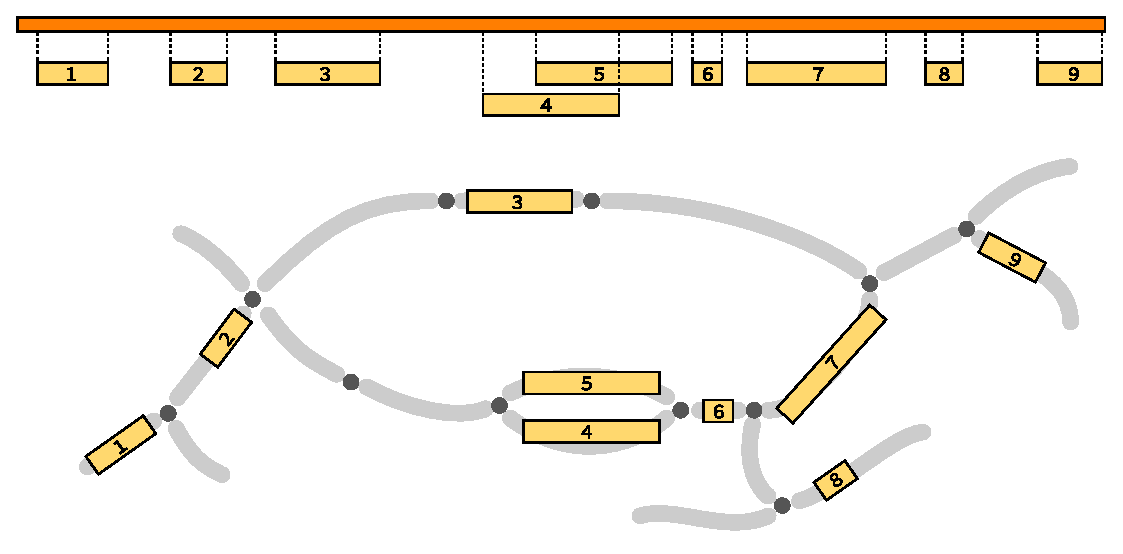
\includegraphics[width=\textwidth]{search.eps}
\end{figure}

\note{
    Теперь о каждом этапе немного подробнее.
    \\ \mbox{} \\
    Первым шагом находятся выравнивания рёбер на последовательности.
    \\ \mbox{} \\
    На рисунке, ораньжемым представлена исправляемая последовательность, серым --- граф сборки, жёлтым с цифрами --- фрагменты рёбер, которые были найдены в последовательности.
}
\end{frame}

% =====================================================================================

\begin{frame}\frametitle{Алгоритм: фильтрация выравниваний}

\begin{figure}
    \includegraphics[width=\textwidth]{filtration.eps}
\end{figure}

\note{
    На следующем шаге мы для каждого выравнивания определяем класс достоверности, а те, что, по нашему мнению, недостаточно надёжно выравнялись, отбрасываем. Такие как, например, короткие рёбра, как 6. Или взаимоисключающие рёбра, как 4 и 5. Или с низким качеством совпадения, как 3. Или выравнивания, которые представляют лишь небольшую часть ребра, как 8. Тем не менее, мы предполагаем, что граф может отличаться своей структурой от последовательности, и поэтому иногда принимаем частичное выравнивание, как в случае 2.
    \\ \mbox{} \\
    Оставшиеся рёбра в выравниваниях будем назвать якорями. Так как якоря мы с учётом класса достоверности считаем верной информацией на следующих шагах, нужно быть очень аккуратными в их выборе. Таким образом, у нас есть около 10и метрик, по которым мы фильтруем.
}
\end{frame}

% =====================================================================================

\begin{frame}\frametitle{Алгоритм: реконструкция заполняющих путей}

\begin{figure}
    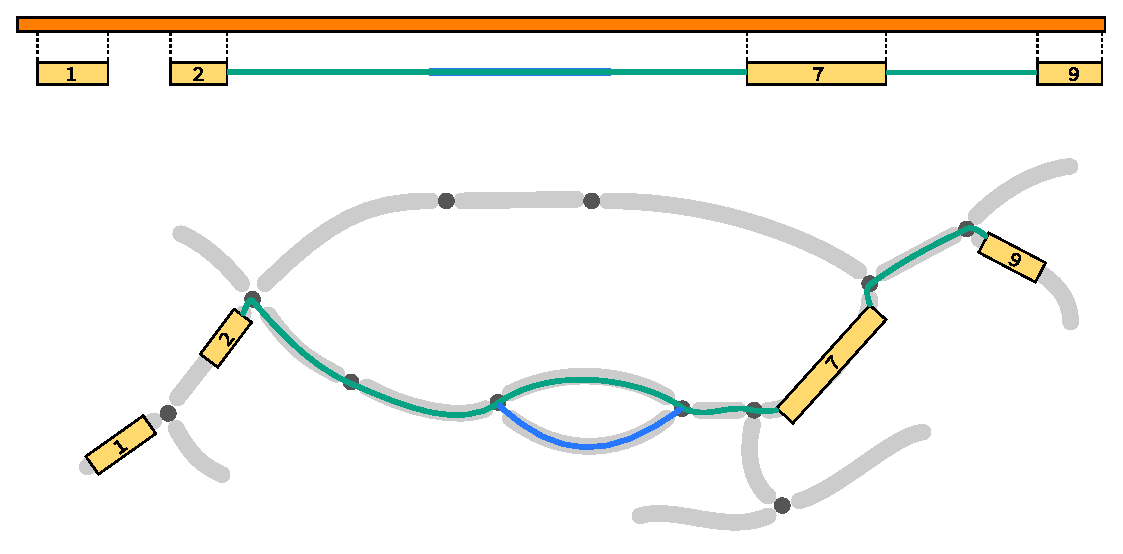
\includegraphics[width=\textwidth]{filling.eps}
\end{figure}

\note{
    После того, как мы оставили достаточно надёжные якоря, хочется как-то покрыть оставшиеся части последовательности рёбрами графа. Чтобы сделать это, между каждыми двумя соседними якорями самого достоверного класса мы ищем все пути в графе, которые довольно похожи на фрагмент последовательности между этими якорями. Очень часто таких путей больше одного, как, например, между рёбрами 3 и 7. В этом случаю, мы выберим либо однозначно лучший путь, либо найдём общие одинаковые фрагменты, ими исправим, а в отличающихся частях трогать ничего не будем, тем самым какбы смешаем пути. Если между парой соседних якорей мы не сформировали заменитель, то для этого фрагмента добавляются якоря следующего уровня достоверности, и поиск происходит вновь с их учётом.
    \\ \mbox{} \\
    Так как в геномах есть довольно много похожих фрагментов, а в метагеномных сборках часто встречаются похожие организмы, высока вероятность выбрать неправильный заполняющий путь и исправить то, что ошибкой не является. Поэтому, в частности, даже когда есть единственный путь между двумя якорями, мы можем посчитать его недостаточно хорошим, чтобы принять.
}
\end{frame}
% =====================================================================================
\begin{frame}\frametitle{Может можно проще?}

\begin{itemize}
    \item Взять какой-нибудь выравниватель на граф
    \begin{itemize}
        \item Например, GraphAligner
    \end{itemize}
    \item По-умному смешать найденные пути
\end{itemize}

\note{
    Можно заметить, что решение довольно похоже на решение задачи выравнивания последовательностей на граф (т.е. нахождение как можно более длинных путей в графе, которые соответствуют фрагментам последовательностей). Кажется, что отличие лишь в том, что мы дополнительно по-умному смешиваем пути между якорями на уровне нуклеотидов. Тогда давайте возьмём какой-нибудь существующий выравниватель на граф, и найденные им пути также по-умному смешаем!
}
\end{frame}
% =====================================================================================
\begin{frame}\frametitle{Вставки и удаления, альтернативный алгоритм}
\begin{figure}[h!]
    \centering
    \include{tables/mix.indels_for_preso.tex}
    % \caption{Вставки и удаления в метагеноме Zymo для основного и альтернативного алгоритма}
    % \label{fig:indels_mix}
\end{figure}

\note{
Оказывается, что так просто сделать нельзя, потому что задачи всё же отличаются. Например, мы можем не взять единственный найденный довольно похожий путь, потому что сочтём его недостаточно хорошим. И вот проверка гипотезы на практике. Был взят метагеном Zymo и выравниватель GraphAligner, который сейчас является одним из лучших инструментов для выравнивания на граф. Столбец без номера --- бактерии метагенома; с цифрой 1 --- сборка ассемлером Flye без коррекции; 2ой --- с нашей коррекцией, 3й --- с коррекцией на основе смешивания путей GraphAligner'a.
\\ \mbox{} \\
Для вставок и удалений картина выглядит не так уж и плохо...
}
\end{frame}
% =====================================================================================
\begin{frame}\frametitle{Замены, альтернативный алгоритм}
\begin{figure}[h!]
    \centering
    \include{tables/mix.mismatches_for_preso.tex}
    % \caption{Замены в метагеноме Zymo для основного и альтернативного алгоритма}
    % \label{fig:mismatches_mix}
\end{figure}

\note{
Но для замен всё куда печальнее.
\\ \mbox{} \\
Обратите внимание на Salmonella enterica. Это связано с тем, что найденные пути прошлись по похожим рёбрам другой бактерии.
}
\end{frame}
% =====================================================================================
\begin{frame}\frametitle{Апробация: схема сравнения}
\begin{figure}[h]
    \centering
    \resizebox{\columnwidth}{!}{
\begin{tikzpicture}[
    every node/.style={
        draw=black,
        anchor=west,
        minimum height=1cm,
        align=center,
        rounded corners 
        }, 
    font=\small
    ]
    \begin{scope}[on grid]

        \node (cor1) {коррекция длинных\\ридов};
        \node (assembly) [right = 1cm of cor1.east] {сборка из длинных\\ридов};
        \node (cor2) [right = 1cm of assembly.east] {коррекция контигов сборки\\из длинных ридов};
        \node[ellipse, inner sep=0pt] (long reads) [above = 2cm of cor1] {длинные риды};
        \node[ellipse, inner sep=0pt] (graph) [above right = 2cm and 2cm of assembly] {граф сборки из коротких ридов};

    \end{scope}

    \path[->]
    (cor1) edge (assembly)
    (assembly) edge (cor2)
    ;
    \path[->, dashed]
    (long reads) edge (cor1)
    (graph) edge (cor1) edge (cor2)
    ;
\end{tikzpicture}
    }
% \caption{Процесс раздельной сборки из коротких и длинных ридов начинается с получения графа сборки. Затем, опционально, длинные риды можно подвергнуть коррекции, после чего из них происходит непосредственно сборка генома, контиги которой также можно опционально попытаться исправить.}
% \label{fig:common_pipeline}
\end{figure}
\note{
    На рисунке показана общая схема проведения сборки раздельно из длинных и коротких ридов. Она начинается с получения графа сборки из коротких ридов. Затем, опционально, длинные риды можно подвергнуть коррекции, после чего из них происходит непосредственно сборка генома, контиги которой также можно опционально попытаться исправить.
    \\ \mbox{} \\
    В ходе апробации используются три варианта сравнения: с коррекцией только длинных ридов, только контигов, и одновременно как длинных ридов, так и контигов.
    \\ \mbox{} \\
    Среди инструментов, которые исправляют длинные риды при помощи коротких ридов, последним вышедшим (2021 г.) и одним из лучших является Ratatosk, поэтому сравнительный анализ будет приведён именно с ним.
    }
\end{frame}
% =====================================================================================
\begin{frame}\frametitle{Апробация: Симулированные данные}
\begin{figure}[h!]
    \centering
    \include{tables/base20.general_for_preso.tex}
\end{figure}

\note{
    \footnotesize
    Здесь представлен результат сравнения на симулированном метагеноме из 20 бактерий.
    \\ \mbox{} \\
    Первой метрикой является покрытие генома. Это процент нуклеотидов генома, которые покрыты контигами. Во всех случаях здесь он примерно одинаковый, а значит была проведена именно коррекция, а не просто часть генома была потеряна.
    \\ \mbox{} \\
    Затем идут структурные ошибки. Если просто, то если два больших фрагмента контига соединено, а в геноме они находятся в разных местах, то это структурная ошибка.
    \\ \mbox{} \\
    Далее идёт среднее количество замен, вставок и удалений символов из генома на 100'000 единиц длины.
    \\ \mbox{} \\
    1ый столбец --- проведена сборка ассемблером Flye без применения коррекций. 2ой --- Ratatosk исправляет контиги. 3ий --- Ratatosk исправляет риды. 4ый --- мы исправляем контиги. 5ый --- Ratatosk исправляет риды, а мы контиги. И 6ой --- Ratatosk исправляет как риды, так и контиги.
    \\ \mbox{} \\
    Видно, что при одиночной коррекции наш алгоритм лучший по вставкам и удалениям, хотя по заменам немного проигрывает. Однако совместная работа с Ratatosk даёт результат сборки в два раза лучше любого другого.
    }
\end{frame}
% =====================================================================================
\begin{frame}\frametitle{Апробация: Bmok12}
\begin{figure}[h!]
    \centering
    \resizebox{0.8\columnwidth}{!}{
\begin{adjustbox}{center}
\begin{tabular}{|l||c|c|c|c|c|c|}
\hline
& 1 & 2 & 3 & 4 & 5 & 6 \\
\hline
\hline
Покрытие генома & \cellcolor[RGB]{252, 232, 232} 62.40 & \cellcolor[RGB]{252, 232, 232} 62.36 & \cellcolor[RGB]{232, 232, 252} 64.43 & \cellcolor[RGB]{252, 232, 232} 62.41 & \cellcolor[RGB]{232, 232, 252} 64.45 & \cellcolor[RGB]{232, 232, 252} 64.40 \\
\hline
Структурные ошибки & \cellcolor[RGB]{227, 227, 252} 72 & \cellcolor[RGB]{237, 237, 253} 77 & \cellcolor[RGB]{247, 182, 182} 129 & \cellcolor[RGB]{227, 227, 252} 72 & \cellcolor[RGB]{253, 237, 237} 99 & \cellcolor[RGB]{235, 71, 71} 145 \\
\hline
Замены на 100kbp & \cellcolor[RGB]{235, 71, 71} 342.69 & \cellcolor[RGB]{205, 205, 249} 127.27 & \cellcolor[RGB]{250, 209, 209} 203.6 & \cellcolor[RGB]{223, 223, 251} 144.39 & \cellcolor[RGB]{246, 246, 254} 166.3 & \cellcolor[RGB]{254, 246, 246} 180.82 \\
\hline
Вставки и удаления на 100kbp & \cellcolor[RGB]{235, 71, 71} 654.71 & \cellcolor[RGB]{253, 237, 237} 61.02 & \cellcolor[RGB]{245, 168, 168} 88.76 & \cellcolor[RGB]{227, 227, 252} 41.56 & \cellcolor[RGB]{200, 200, 249} 28.6 & \cellcolor[RGB]{237, 237, 253} 46.28 \\
\hline
\end{tabular}
\end{adjustbox}
}

\end{figure}
\note{
    Из настоящих метагеномов первым будет Bmok12 --- это метагеном из, внезапно, 11 организмов. 
    \\ \mbox{} \\
    Видно, что результат хуже всех после коррекции ридов Ratatosk, который ещё привёл к существенному повышению количества структурных ошибок.
    \\ \mbox{} \\
    Лучшим по вставкам и удалениям при одиночной коррекции является наш наша алгоритм, лишь немного проигрывая по заменам. Совместная работа нашего алгоритма и Ratatosk для замен в этот раз не является лучшей, однако до вставкам и удалениям она обходит всех минимум на 20\%.
}
\end{frame}
% =====================================================================================
\begin{frame}\frametitle{Апробация: Zymo}
\begin{figure}[h!]
    \centering
    \resizebox{0.8\columnwidth}{!}{
\begin{minipage}{0.91\textwidth}
\begin{adjustbox}{center}
\begin{tabular}{|l||c|c|c|c|c|c|}
\hline
 & raw & ratatosk & ratatosk & our & ratatosk & ratatosk \\
 & flye & contigs & reads & contigs & and we & ratatosk \\
\hline
\hline
Покрытие генома & \cellcolor[RGB]{227, 227, 252} 97.12 & \cellcolor[RGB]{237, 237, 253} 97.09 & \cellcolor[RGB]{252, 227, 227} 96.93 & \cellcolor[RGB]{232, 232, 252} 97.11 & \cellcolor[RGB]{251, 223, 223} 96.91 & \cellcolor[RGB]{253, 241, 241} 96.98 \\
\hline
Структурные ошибки & \cellcolor[RGB]{253, 241, 241} 69 & \cellcolor[RGB]{246, 246, 254} 68 & \cellcolor[RGB]{245, 163, 163} 72 & \cellcolor[RGB]{223, 223, 251} 67 & \cellcolor[RGB]{248, 191, 191} 71 & \cellcolor[RGB]{205, 205, 249} 66 \\
\hline
Замены на 100kbp & \cellcolor[RGB]{235, 71, 71} 109.39 & \cellcolor[RGB]{235, 71, 71} 60.51 & \cellcolor[RGB]{253, 237, 237} 42.98 & \cellcolor[RGB]{227, 227, 252} 34.02 & \cellcolor[RGB]{227, 227, 252} 34.58 & \cellcolor[RGB]{237, 237, 253} 36.09 \\
\hline
Вставки и удаления на 100kbp & \cellcolor[RGB]{235, 71, 71} 214.49 & \cellcolor[RGB]{235, 71, 71} 47.68 & \cellcolor[RGB]{227, 227, 252} 21.3 & \cellcolor[RGB]{253, 241, 241} 22.22 & \cellcolor[RGB]{48, 48, 232} \white{18.07} & \cellcolor[RGB]{241, 241, 253} 21.64 \\
\hline
\end{tabular}
\end{adjustbox}
\end{minipage}
}

\end{figure}
\note{
    Zymo --- это синтетическое сообщество, состоящее из сместьи девяти бактериальных и дрожжевых организмов.
    \\ \mbox{} \\
    Здесь видно, что Ratatosk хуже всех справился с коррекцией контигов. Лучшим по заменам является наш наша коррекция, а кооперация усилий даёт лучший результат по вставкам и удалениям.
}
\end{frame}
% =====================================================================================
            

\begin{frame}\frametitle{Заключение}
\begin{itemize}
    \item Сформированы критерии фильтрации выравниваний рёбер графа на последовательности.
    \item Разработан алгоритм исправления ошибок за пределами выравненных рёбер.
    \item Разработан алгоритм переноса полученных путей в графе обратно в последовательности.
    \item Итоговый алгоритм реализован в виде отдельного инструмента.
    \begin{itemize}
        \item Реализация выполнена на языке C++ и является подпроектом для ассемблера SPAdes.
        \item \begin{sloppypar} Исходный код SPAdes доступен по ссылке: \mbox{\url{https://github.com/ablab/spades/}}. Реализованный инструмент будет доступен начиная с версии 3.17. \end{sloppypar}
    \end{itemize}
    \item Проведена апробация алгоритма на симулированных и реальных данных.
    \begin{itemize}
        \item Сравнимый и лучший результат по сравнению с коррекцией ридов и сборок существующими решениями.
        \item Кооперация даёт существенно лучший результат.
    \end{itemize}

\end{itemize}

\note{
Итак, в ходе данной работы были достигнуты следующие результаты. Сформированы критерии фильтрации выравниваний рёбер графа на последовательности. Разработан алгоритм исправления ошибок за пределами выравненных рёбер. Разработан алгоритм переноса полученных путей в графе обратно в последовательности. Итоговый алгоритм реализован в виде отдельного инструмента на языке C++ в качестве подпроекта для ассемблера SPAdes. Он будет появится в открытом доступе начиная со следующего релиза. Также проведена апробация на симулированных и реальных данных. При этом исправление метагеномных сборок низкого качества даёт сравнимый и лучший результат по сравнению с коррекцией ридов и сборок существующими решениями. А кооперация с существующими решениями даёт существенно лучший результат.
}
\end{frame}

% =====================================================================================

\end{document}